%
% Main document
% ===========================================================================
% This is part of the document "Project documentation template".
% Authors: brd3, kaa1
%

\title{BFH Modul BTI7311 Informatik Seminar}

%---------------------------------------------------------------------------
\documentclass[
	a4paper,					% paper format
	10pt,							% fontsize
	twoside,					% double-sided
	openright,				% begin new chapter on right side
	notitlepage,			% use no standard title page
	parskip=half,			% set paragraph skip to half of a line
]{scrreprt}					% KOMA-script report
%---------------------------------------------------------------------------

\raggedbottom
\KOMAoptions{cleardoublepage=plain}			% Add header and footer on blank pages


% Load Standard Packages:
%---------------------------------------------------------------------------
\usepackage[standard-baselineskips]{cmbright}

\usepackage[ngerman]{babel}							% german hyphenation
\usepackage[utf8x]{inputenc} 						% UTF-8
\usepackage[T1]{fontenc}							% hyphenation of words with ä,ö and ü
\usepackage{textcomp}								% additional symbols
\usepackage{ae}										% better resolution of Type1-Fonts 
\usepackage{fancyhdr}								% simple manipulation of header and footer 
\usepackage{etoolbox}								% color manipulation of header and footer
\usepackage{graphicx}                      			% integration of images
\usepackage{float}									% floating objects
\usepackage{caption}								% for captions of figures and tables
\usepackage{booktabs}								% package for nicer tables
\usepackage{tocvsec2}								% provides means of controlling the sectional numbering
\usepackage{listings}												
\usepackage[onehalfspacing]{setspace}				% Linespacing 1.5
%---------------------------------------------------------------------------

% Load Math Packages
%---------------------------------------------------------------------------
\usepackage{amsmath}                    	   	% various features to facilitate writing math formulas
\usepackage{amsthm}                       	 	% enhanced version of latex's newtheorem
\usepackage{amsfonts}                      		% set of miscellaneous TeX fonts that augment the standard CM
\usepackage{amssymb}							% mathematical special characters
\usepackage{exscale}							% mathematical size corresponds to textsize
%---------------------------------------------------------------------------

% Package to facilitate placement of boxes at absolute positions
%---------------------------------------------------------------------------
\usepackage[absolute]{textpos}
\setlength{\TPHorizModule}{1mm}
\setlength{\TPVertModule}{1mm}
%---------------------------------------------------------------------------					
			
% Definition of Colors
%---------------------------------------------------------------------------
\RequirePackage{color}                          % Color (not xcolor!)
\definecolor{linkblue}{rgb}{0,0,0.8}            % Standard
\definecolor{darkblue}{rgb}{0,0.08,0.45}        % Dark blue
\definecolor{bfhgrey}{rgb}{0.41,0.49,0.57}      % BFH grey
%\definecolor{linkcolor}{rgb}{0,0,0.8}     			% Blue for the web- and cd-version!
\definecolor{linkcolor}{rgb}{0,0,0}        			% Black for the print-version!
%---------------------------------------------------------------------------

% Hyperref Package (Create links in a pdf)
%---------------------------------------------------------------------------
\usepackage[
	pdftex,ngerman,bookmarks,plainpages=false,pdfpagelabels,
	backref = {false},										% No index backreference
	colorlinks = {true},                  % Color links in a PDF
	hypertexnames = {true},               % no failures "same page(i)"
	bookmarksopen = {true},               % opens the bar on the left side
	bookmarksopenlevel = {0},             % depth of opened bookmarks
	pdftitle = {Verteilte Netzwerk-Algorithmen},	   	% PDF-property
	pdfauthor = {Adrian Bärtschi},        					  % PDF-property
	pdfsubject = {LaTeX Template},        % PDF-property
	linkcolor = {linkcolor},              % Color of Links
	citecolor = {linkcolor},              % Color of Cite-Links
	urlcolor = {linkcolor},               % Color of URLs
]{hyperref}
%---------------------------------------------------------------------------
% Set up page dimension
%---------------------------------------------------------------------------
\usepackage{geometry}
\geometry{
	a4paper,
	left=28mm,
	right=15mm,
	top=30mm,
	headheight=20mm,
	headsep=10mm,
	textheight=242mm,
	footskip=15mm
}
%---------------------------------------------------------------------------

% Makeindex Package
%---------------------------------------------------------------------------
\usepackage{makeidx}                         		% To produce index
\makeindex                                    	% Index-Initialisation
%---------------------------------------------------------------------------

% Glossary Package
%---------------------------------------------------------------------------
% the glossaries package uses makeindex
% if you use TeXnicCenter do the following steps:
%  - Goto "Ausgabeprofile definieren" (ctrl + F7)
%  - Select the profile "LaTeX => PDF"
%  - Add in register "Nachbearbeitung" a new "Postprozessoren" point named Glossar
%  - Select makeindex.exe in the field "Anwendung" ( ..\MiKTeX x.x\miktex\bin\makeindex.exe )
%  - Add this [ -s "%tm.ist" -t "%tm.glg" -o "%tm.gls" "%tm.glo" ] in the field "Argumente"
%
% for futher informations go to http://ewus.de/tipp-1029.html
%---------------------------------------------------------------------------
\usepackage[nonumberlist]{glossaries}
\makeglossaries
\newglossaryentry{BibTeX}{name={BibTeX},description={Programm zur Erstellung von Literaturangaben und -verzeichnissen in \TeX- oder \LaTeX-Dokumenten}}
\newglossaryentry{StwVrz}{name={Stichwortverzeichnis},description={Verzeichnis mit Stichworten aus dem Text}}
%---------------------------------------------------------------------------

% Styles for Code Listings
%---------------------------------------------------------------------------
\definecolor{codegreen}{rgb}{0,0.6,0}
\definecolor{codegray}{rgb}{0.5,0.5,0.5}
\definecolor{backcolour}{rgb}{0.95,0.95,0.92}

%Code listing style for Pseudocode
\lstdefinestyle{pseudocode}{
  backgroundcolor=\color{backcolour},   commentstyle=\color{codegreen},
  numberstyle=\tiny\color{codegray},
  basicstyle=\footnotesize,
  breakatwhitespace=false,         
  breaklines=true,                 
  captionpos=b,                    
  keepspaces=true,                 
  numbers=left,                    
  numbersep=5pt,                  
  showspaces=false,                
  showstringspaces=false,
  showtabs=false,                  
  tabsize=2
}

% Intro:
%---------------------------------------------------------------------------
\begin{document}                              	% Start Document
\settocdepth{section}														% Set depth of toc
\pagenumbering{roman}														
%---------------------------------------------------------------------------

\providecommand{\titel}{Verteilte Netzwerk-Algorithmen}		%  Hier den Titel des Berichts/Thesis eingeben					% Titel der Arbeit aus Datei titel.tex lesen
\providecommand{\versionnumber}{1.0}			%  Hier die aktuelle Versionsnummer eingeben
\providecommand{\versiondate}{09.05.2015}		%  Hier das Datum der aktuellen Version eingeben				% Versionsnummer und -datum aus Datei version.tex lesen

% Set up header and footer
%---------------------------------------------------------------------------
\makeatletter
\patchcmd{\@fancyhead}{\rlap}{\color{bfhgrey}\rlap}{}{}		% new color of header
\patchcmd{\@fancyfoot}{\rlap}{\color{bfhgrey}\rlap}{}{}		% new color of footer
\makeatother

\fancyhf{}																		% clean all fields
\fancypagestyle{plain}{												% new definition of plain style	
	\fancyfoot[OR,EL]{\footnotesize \thepage} 	% footer right part --> page number
	\fancyfoot[OL,ER]{\footnotesize \titel, Version \versionnumber, \versiondate}	% footer even page left part 
}

\renewcommand{\chaptermark}[1]{\markboth{\thechapter.  #1}{}}
\renewcommand{\headrulewidth}{0pt}				% no header stripline
\renewcommand{\footrulewidth}{0pt} 				% no bottom stripline

\pagestyle{plain}
%---------------------------------------------------------------------------


% Title Page and Abstract
%---------------------------------------------------------------------------
%
% Project documentation template
% ===========================================================================
% This is part of the document "Project documentation template".
% Authors: brd3, kaa1
%

\begin{titlepage}


% BFH-Logo absolute placed at (28,12) on A4 
% Actually not a realy satisfactory solution but working.
%---------------------------------------------------------------------------
\setlength{\unitlength}{1mm}
\begin{textblock}{20}[0,0](28,12)
	
\includegraphics[scale=1.0]{bilder/BFH_Logo_B.png}
\end{textblock}
\color{black}

% Institution / Titel / Untertitel / Autoren / Experten:
%---------------------------------------------------------------------------
\begin{flushleft}

\vspace*{21mm}

\fontsize{26pt}{40pt}\selectfont 
\titel 				\\							% Titel aus der Datei vorspann/titel.tex lesen
\vspace{2mm}

\fontsize{16pt}{24pt}\selectfont\vspace{0.3em}
%Hier steht ein Untertitel 			\\							% Untertitel eingeben
\vspace{5mm}

\fontsize{10pt}{12pt}\selectfont
\textbf{Bericht Modul BTI7311 Informatik Seminar} \\									% eingeben
\vspace{7mm}


\begin{textblock}{150}(28,225)
\fontsize{10pt}{17pt}\selectfont
\begin{tabbing}
xxxxxxxxxxxxxxx\=xxxxxxxxxxxxxxxxxxxxxxxxxxxxxxxxxxxxxxxxxxxxxxx \kill
Studiengang:	\> Informatik	\\			% Namen eingeben
Autor:			\> Adrian Bärtschi		\\					% Namen eingeben
Betreuer:		\> Peter Schwab		\\					% Namen eingeben
Datum:			\> \versiondate					\\		% aus Datei vorspann/version.tex lesen
\end{tabbing}

\end{textblock}
\end{flushleft}

\begin{textblock}{150}(28,280)
\noindent 
\color{bfhgrey}\fontsize{9pt}{10pt}\selectfont
Berner Fachhochschule | Haute école spécialisée bernoise | Bern University of Applied Sciences
\color{black}\selectfont
\end{textblock}


\end{titlepage}

%
% ===========================================================================
% EOF
%		% activate for Titelseite ohne Bild
% Versionenkontrolle :
% -----------------------------------------------

\begin{textblock}{180}(15,150)
\color{black}
\begin{huge}
Versionen
\end{huge}
\vspace{10mm}

\fontsize{10pt}{18pt}\selectfont
\begin{tabbing}
xxxxxxxxxxx\=xxxxxxxxxxxxxxx\=xxxxxxxxxxxxxx\=xxxxxxxxxxxxxxxxxxxxxxxxxxxxxxxxxxxxxxxxxxxxxxx \kill
Version	\> Datum	\> Status		\> Bemerkungen		\\
0.1	\> 28.03.2015	\> Entwurf		\> Setup Template	\\	
0.2	\> 26.04.2015	\> Entwurf		\> Disposition, Einleitung	\\	
0.3	\> 05.05.2015	\> Entwurf		\> Inhalte	\\	
1.0	\> 09.05.2015	\> Final		\> Fazit, Korrekturen, Abschluss	\\	

\end{tabbing}

\end{textblock}
\cleardoubleemptypage
\setcounter{page}{1}
\cleardoublepage
\phantomsection 
\cleardoubleemptypage
%---------------------------------------------------------------------------

% Table of contents
%---------------------------------------------------------------------------
\tableofcontents
\cleardoublepage
%---------------------------------------------------------------------------

% Main part:
%---------------------------------------------------------------------------
\pagenumbering{arabic}

\chapter{Einleitung}
\label{chap:einleitung}

Um in verteilten, miteinander verbunden Systemen Information zu gewinnen, werden Algorithmen mit speziellen Eigenschaften benötigt. Diese Algorithmen laufen meistens gleichzeitig auf den verschiedenen Knoten eines Netzwerks. Die einzelnen Teilprogramme kennen dabei nicht das ganze Netz, sondern lediglich ihre direkten Nachbarn.
Netzwerkalgorithmen müssen also autonom auf den Knoten laufen können und dürfen nicht auf feste Grössen (zum Beispiel Anzahl Netzwerkteilnehmer) angewiesen sein. Es muss dazu sichergestellt sein, dass Entscheidungen und Berechnungsresultate alle gewünschten Knoten erreichen und dass sich so eine gewisse Konsistenz bilden kann.

Typische Schwierigkeiten von verteilte Algorithmen sind das Koordinieren der einzelnen Prozesse bei teilweisen Ausfällen und unzuverlässigen Verbindungen.

Praktische Anwendungen von verteilten Algorithmen sind zum Beispiel Routing, Spanning Trees oder Transaktionssteuerung bei verteilten Datenbanken. 
\chapter{Grundlagen}
\label{chap:glundlagen}


\section{Message-Passing Modell}

Um Abläufe in verteilten System zu beschreiben, wird das Message-Passing Modell genutzt. Dabei wird das Netzwerk als Graph abgebildet. Prozessoren stellen dabei die Knoten dar und direkte Verbindungen werden durch die dazugehörigen Kanten repräsentiert. Die Teilnehmer kommunizieren untereinander, indem sie Messages versenden und empfangen (in der Praxis z. Bsp. TCP/IP Pakete). Dazu muss jeder Knoten eindeutig identifizierbar sein, beispielweise via MAC-Adresse, und die direkten Nachbarn müssen bekannt sein.

\begin{figure}[h]
	\centering
		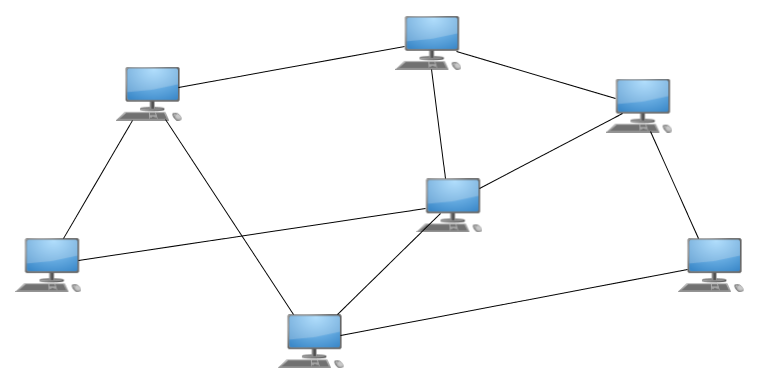
\includegraphics[width=0.6\textwidth]{bilder/network.png}
	\caption{\label{fig:network}Schematische Darstellunge eines Netzwerks als Graph}
\end{figure}


Teilweise ist auch noch die Gesamtanzahl Teilnehmer in Netzwerk bekannt, häufig ist dies aber aufgrund der Grösse und Dynamik nicht möglich.\\
In verteilten Systemen kann es vorkommen, dass sich die Struktur ändert, sich neue Teilnehmer anmelden oder dass Knoten und Verbindungen sich fehlerhaft verhalten oder ganz ausfallen. Verteilte Algorithmen müssen grundsätzlich auch mit solchen Problemen umgehen können, in diesem Bericht wird aber darauf nicht näher eingegangen.\\
Bei den behandelten Anwendungen wird angenommen, dass sich das Netzwerk zur Laufzeit nicht ändert und dass alle Teilemhmer und Verbindungen ohne Fehler funktionieren.


Ein wichtiger Aspekt des Message-Passings ist die Synchronisation der Prozesse. Es gibt dabei verschiedene Ansätze:

\textbf{Synchrones Modell:}
Beim synchronen Modell geht man davon aus, dass bei jedem Prozessor ein interner Timer läuft. Die Timer laufen alle genau gleich schnell und die Prozessoren benötigen für die gleiche Aufgabe die gleiche Zeit. Ausserdem wird angenommen, dass das Versenden von Nachrichten immer die gleiche Zeit dauert, egal über welche Verbindung dies geschieht.

\textbf{Asynchrones Modell:}
In asynchronen Modellen gibt es keinen einheitlichen Takt unter den Prozessoren. Man muss annehmen, dass die Knoten unterschiedlich schnell arbeiten. Um trotzdem verteilte Algorithmen einsetzten zu können, wird bei jedem Knoten eine Queue eingeführt, mit welcher ankommende Nachrichten zwischengespeichert werden.

\begin{figure}[H]
	\centering
		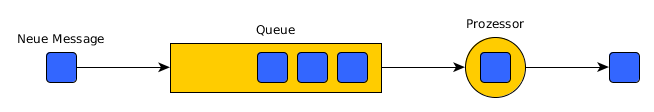
\includegraphics[width=0.6\textwidth]{bilder/queue.png}
	\caption{\label{fig:network}Prozessor mit first-in-first-out Queue}
\end{figure}


Die meisten Netzwerke in der Praxis orientieren sich eher am asynchronen Modell. Gewisse Aspekte aus dem synchronen Modell, wie zum Beispiel ein Timeout falls die Übertragung zu lange dauert, sind jedoch auch häufig anzutreffen. Netzwerkalgorithmen für synchrone Netzwerke können meistens für das asynchrone Modell erweitert werden. Ein Algorithmus, der für ein asynchrones Netzwerk funktioniert, läuft mit Sicherheit auch bei in einen synchronen Netz.


\section{Einheiten für die Komplexität der Algorithmen}
Bei normalen, sequenziellen Algorithmen sind für die Ermittlung der Komplexität meistens die Laufzeit und der benötigte Speicherplatz relevant. Bei verteilten Systemen reichen diese Kriterien nicht mehr aus, um einen Algorithmus beurteilen zu können.
Folgende Kennwerten spielen eine Rolle:

\begin{itemize}
\item \textbf{Anzahl Berechnungsrunden (Computational Rounds)}\\
Die Algorithmen kommen nach einer gewissen Anzahl Berechnungsrunden zum Ergebnis. Bei synchronen Algorithmen kann man die Anzahl Ticks der Timer als Messgrösse benutzen. Im asynchronen Modell laufen die Algorithmen häufig in Wellen von Events durch das Netz. Hier kann somit die Anzahl Wellen eine relevante Grösse sein.

\item \textbf{Benötigter Speicherplatz}\\
Es gibt zwei Kenngrössen für den benötigen Speicher des Algorithmus. Zum einen kann der lokale Speicherplatz auf einem Knoten eine wichtige Information sein. Zum anderen kann über das ganze Netz die Gesamtsumme des benötigten Speichers ausgewertet werden.

\item \textbf{Lokale Laufzeit}\\
Die lokale Laufzeit der Algorithmen auf den Knoten ist auch in verteilten System noch eine wichtige Grösse. Es kann vorkommen, dass die Knoten unterschiedliche Laufzeiten haben, da z. Bsp. Knoten am Rand des Netzes spezielle Aufgaben übernehmen müssen.

\item \textbf{Anzahl und Grösse der Messages}\\
Typischerweise wird analysiert, wie viele Messages für die Ausführung einer Berechnungsrunde versendet werden müssen. Bei Algorithmen mit unterschiedlichen Messagetypen ist auch die Grösse der unterschiedlichen Messages zu beachten.

\end{itemize}

\newpage

\section{Leader Election Ring}
Ein typisches Beispiel eines Netzwerkalgorithmus ist Leader Election. Die Ausgangslage ist ein Ringnetzwerk, bei dem jeder Knoten über eine Nummer identifizierbar ist.\\
Das Ziel ist nun, den Knoten mit der höchsten (oder tiefsten) Nummer zu finden und diese Information im gesamten Ring bekannt zu geben. Somit sollen sich alle Knoten einig sein, welcher als Leader gewählt wurde.\\
Die Knoten kennen lediglich ihre Nummer und den nächsten Knoten, and den sie als einziges Messages senden können.

\begin{figure}[h]
	\centering
		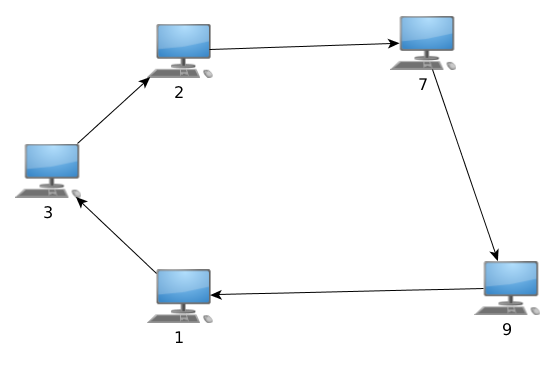
\includegraphics[width=0.5\textwidth]{bilder/ring.png}
	\caption{\label{fig:network}Ausgangslage Leader Election Ring}
\end{figure}

Die Lösung dieses Problems funktioniert nach folgendem Ansatz:

\begin{enumerate}
  	\item Jeder Knoten sendet seine Nummer zum nächsten Knoten
 	\item Wenn eine Nummer empfangen wurde, wird diese mit der eigenen Nummer verglichen
 	\begin{enumerate}
		\item Die grössere der beiden Nummern wird weitergeschickt
        \item Falls die empfangene Nummer die eigenen Nummer ist, ist der Leader gefunden worden
	\end{enumerate}
\end{enumerate}

Es werden zwei verschiedene Messagetypen eingeführt. `Candidate is ...' um einen möglichen Leader dem nächsten Knoten zu melden und `Leader is ...', sobald klar ist, welcher Knoten als Leader bestimmt wurde.
In der ersten Phase werden so lange `Candidate is' Messages versendet, bis die Nummer des Leaders den gesamten Ring durchlaufen hat. Sobald die Message den Ursprungsknoten erreicht hat, wird begonnen `Leader is' Messages zu versenden um die anderen Knoten zu informieren. \\
Dieser Lösungsansatz setzt voraus, dass die Nummern der Knoten eindeutig sind. 

\newpage

\lstset{style=pseudocode}
\begin{lstlisting}[caption=Pseudocode Asynchrone Leader Election in einen Ring Netzwerk]
send Message [Candidate is myId]

finished = false
while not finished
    M = Get Next Message from incoming Queue
    if M is "Candidate is ..." Message then
        if M.id = myId them
            send Message [Leader is myId]
            finished = true
        else
            send Message [Candidate is max(M.id, myId)]
    else
        send M
        finished = true
\end{lstlisting}

Eine Implementation des obigen Algorithmus in Java ist in Anhang \ref{chap:app_leaderElection} zu finden.

Bei einem Ring mit n Knoten sendet in der ersten Phase jeder Knoten n 'Candidate is' Messages. Somit werden in der ersten Phase $O(n^{2})$ Messages versendet.\\
Sobald der Leader bestimmt ist, muss die `Leader is' Message eine komplette Runde durch den Ring absolvieren. In dieser Zeit senden die anderen Knoten weiter `Candidate is' Messages, bis die `Leader is' Message sie erreicht hat. Durchschnittlich versendet jeder Knoten noch \( \frac{n}{2} \) `Candidate is' Messages. Die Message Komplexität des Ring Leader Election Algorithmus entspricht also $O(n^{2})$.



\section{Leader Election Tree} \label{sec_leaderElectionTree}
Für ein Netzwerk das eine Baumstuktur hat, muss der Leader Election Algorithmus natürlich angepasst werden. Der Algorithmus läuft in zwei Phasen ab.
\begin{enumerate}
	\item Die \textbf{Akkumulationsphase} startet bei den externen Knoten (Knoten mit nur einem Nachbarn). Diese senden ihre Nummer an den Nachbar. Jeder Knoten wartet und speichert die eingehenden Nachrichten, bis er von allen ausser einem Nachbarn eine Nachricht erhalten hat. Dann wird die grösste bekannte Nummer an den verbleibenden Knoten gesendet. Sobald ein Knoten von allen Nachbarn Nachrichten erhalten hat, ist der gesamte Baum durchlaufen worden und der verbleibende Knoten kann entscheiden, welcher Teilnehmer als Leader gewählt wird.
    
\begin{figure}[H]
	\centering
		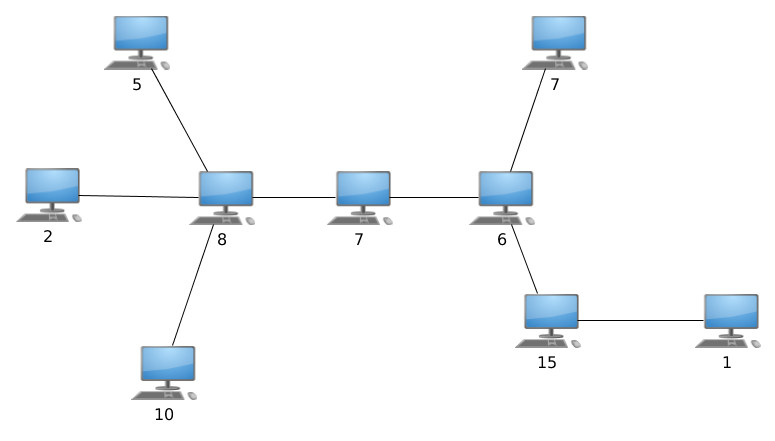
\includegraphics[width=0.6\textwidth]{bilder/leaderElectionTree_1.png}
	\caption{\label{fig:treeLeader_1}Leader Election Tree Ausgangslage}
\end{figure}

\begin{figure}[H]
	\centering
		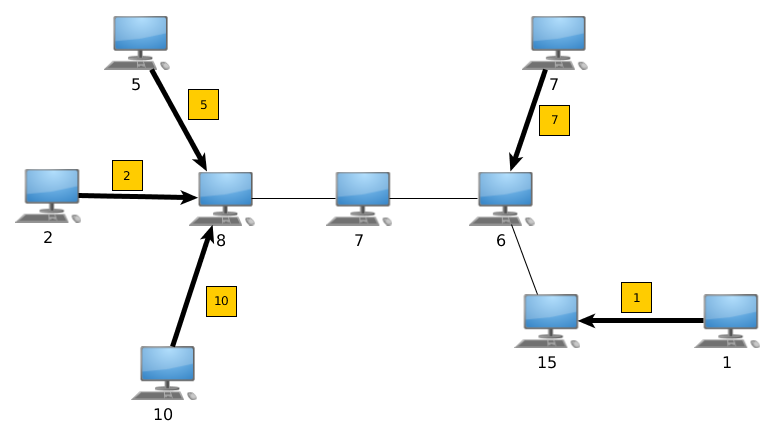
\includegraphics[width=0.6\textwidth]{bilder/leaderElectionTree_2.png}
	\caption{\label{fig:treeLeader_2}Leader Election Tree Accumulation Schritt 1}
\end{figure}

\begin{figure}[H]
	\centering
		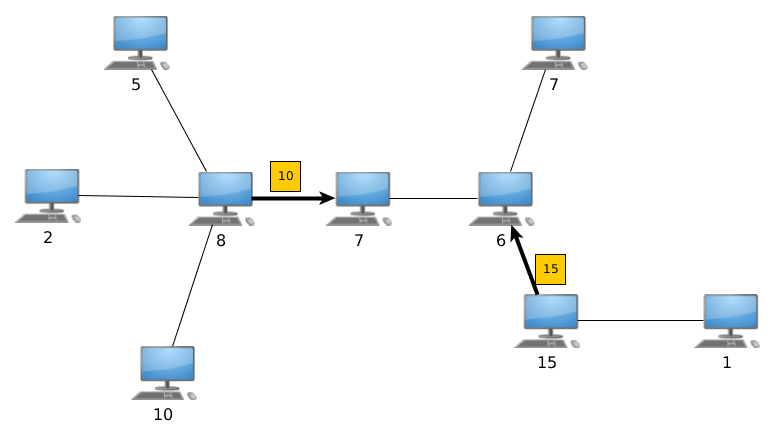
\includegraphics[width=0.6\textwidth]{bilder/leaderElectionTree_3.png}
	\caption{\label{fig:treeLeader_3}Leader Election Tree Accumulation Schritt 2}
\end{figure}

\begin{figure}[H]
	\centering
		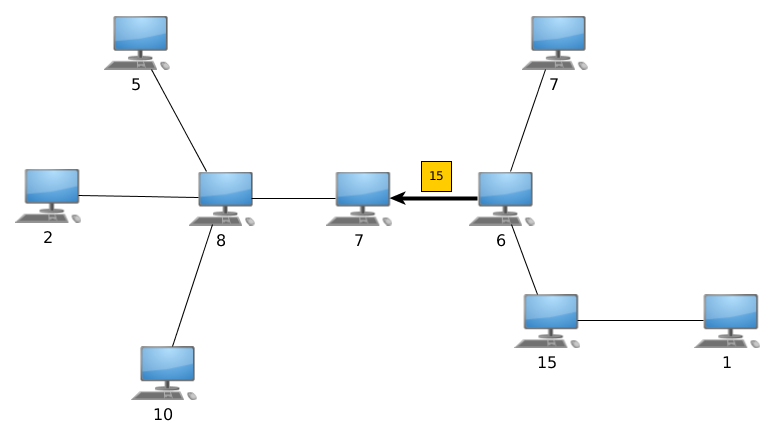
\includegraphics[width=0.6\textwidth]{bilder/leaderElectionTree_4.png}
	\caption{\label{fig:treeLeader_4}Leader Election Tree Accumulation Schritt 3}
\end{figure}
    
    \item Der letzte Node startet nun die \textbf{Broadcastphase}, bei der die Leader Information an jeweils alle Knoten gesendet wird (ausgenonnen vom Nachbarn, von dem die Broadcast Nachricht erhalten wurde).

\begin{figure}[H]
	\centering
		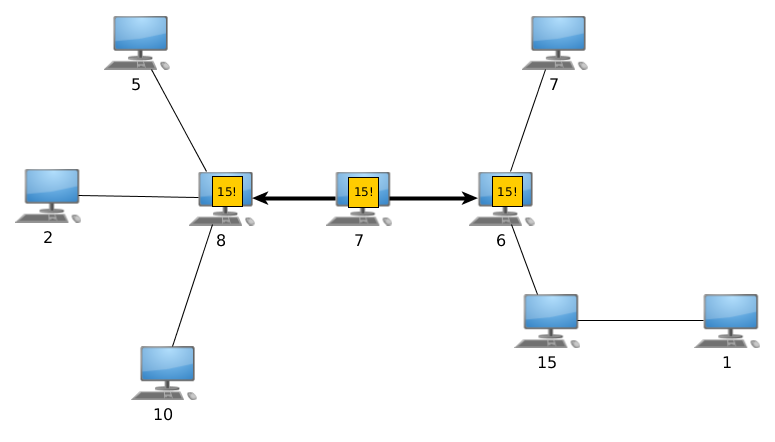
\includegraphics[width=0.6\textwidth]{bilder/leaderElectionTree_5.png}
	\caption{\label{fig:treeLeader_5}Leader Election Tree Broadcast Schritt 1}
\end{figure}

\begin{figure}[H]
	\centering
		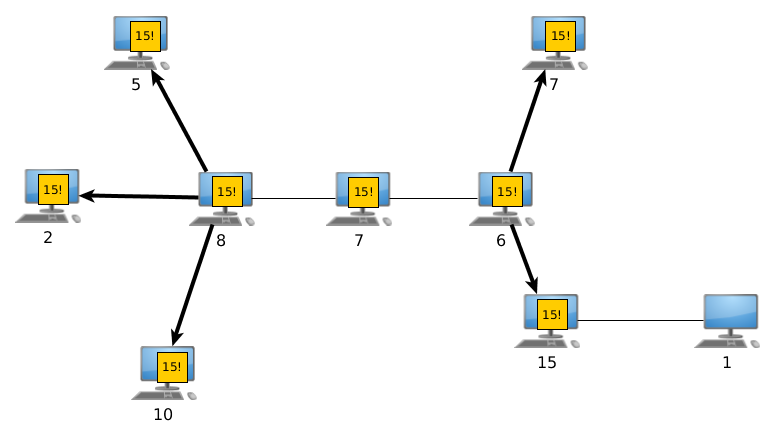
\includegraphics[width=0.6\textwidth]{bilder/leaderElectionTree_6.png}
	\caption{\label{fig:treeLeader_6}Leader Election Tree Broadcast Schritt 2}
\end{figure}

\begin{figure}[H]
	\centering
		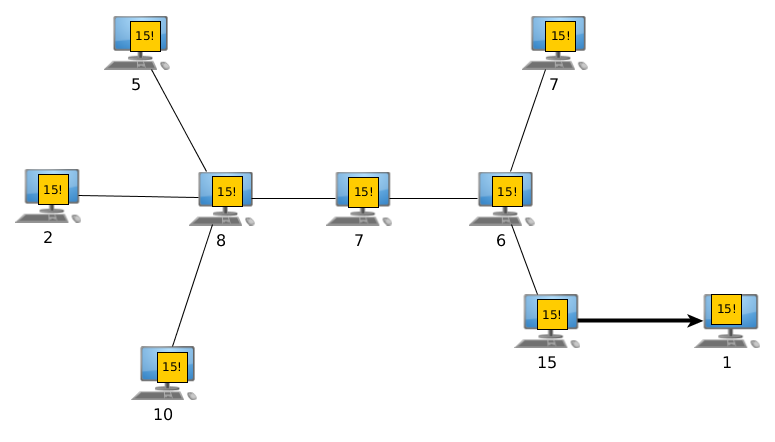
\includegraphics[width=0.6\textwidth]{bilder/leaderElectionTree_7.png}
	\caption{\label{fig:treeLeader_7}Leader Election Tree Broadcast Schritt 3}
\end{figure}

\end{enumerate}

Bei der asynchronen Variante dieses Algorithmus sendet während der Akkumulationsphase jeder Knoten genau eine 'Candidate is'  Nachricht. Für den Broadcast wird schlussendlich an jeden Knoten eine 'Leader is' Message versendet. Die Messages haben eine Grösse von $O(1)$. Somit ist die Message Komplexität bei einem Baum mit n Knoten $O(n)$.


Ein Beispiel für eine praktische Anwendung von Leader Election ist der Clusterverbund von mehreren Servern. Dabei muss ein Server als Leader ermittelt werden, von dem dann koordinative Aufgaben wie Deployment und Logging übernommen werden.



\section{Minimum Spanning Trees}
Der Minimum Spanning Tree eines Graphen ist ein Subgraph, der alle Knoten erreicht und dessen summiertes Gewicht der Kanten minimal ist \cite{wiki:mst}.

\begin{figure}[H]
	\centering
		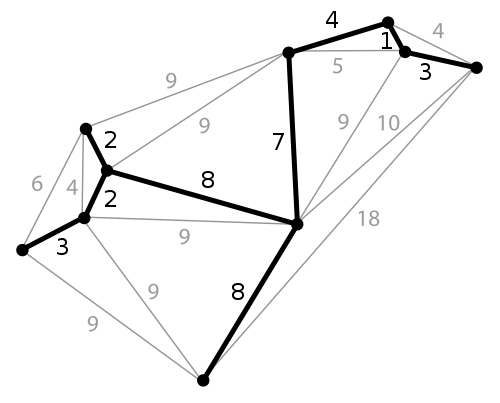
\includegraphics[width=0.5\textwidth]{bilder/500px-Minimum_spanning_tree.png}
	\caption{\label{fig:mst}Beispiel eines Minimum Spanning Trees \cite{wiki:mst}}
\end{figure}

Eine effiziente sequenzielle Lösung für das finden des Minimum Spanning Trees ist der Algorithmus von Baruvka \cite{wiki:boruvka}. Die Idee dabei ist, von jedem Knoten ausgehend Cluster mit dem Nachbarn zu bilden, der über die Kante mit dem kleinsten Gewicht verbunden ist. Der am Schluss entstandenen Graph ist der Minimum Spanning Tree.

Um in verteilten Systemen zu funktionieren, muss der Algorithus angepasst werden. Nachfolged ist die synchrone, verteilte Variante der Minimum Spanning Tree Generierung beschrieben.


\begin{enumerate}
	\item Da die einzelnen Knoten nur ihre direkten Nachbarn kennen, müssen mit Hilfe des Tree Leader Election Algorithmus (siehe Kapitel \ref{sec_leaderElectionTree}) die zusammenhängenden Komponenten bestimmt werden.
    \item Zu jeder zusammenhängenden Komponente muss die Kante gefunden werden mit dem tiefsten Gewicht, die einen neuen Knoten mit der zusammenhängenden Komponente verbindet. Auf jedem Knoten wird nun erneut eine Leader Election durchgeführt, nun mit den angrenzenden Kanten respektiv deren Gewicht.
    \item Dies läuft so lange, bis alle Knoten erschlossen wurden.
\end{enumerate}

In einem Graphen mit n Knoten und m Kanten werden pro Runde $O(m)$ Messsages versendet. Die Anzahl zusammenhängender Komponenten im Graphen halbiert sich mit jeder Runde. Somit gibt es $O(\log{}n)$ Runden, bis der Spanning Tree gefunden wurde. Dies ergibt eine Message Komplexität von $O(m\log{}n)$.

Minimum Spanning Trees werden beispielsweise verwendet, um in einem Netzwerk möglichst effizient eine Nachricht an alle Teilnehmer zu versenden (Broadcast).

\chapter{Routing}
\label{chap:routing}

\section{Broadcast Routing mit Flooding}

Ein einfacher Weg, um eine Nachricht von einem Teilnehmer aus an alle anderen des Netzwerks zu senden, ist Flooding. Der Knoten, der senden möchte, sendet die Nachricht an alle seine Nachbarn. Diese leiten die Nachricht an alle Nachbarn weiter, ausser dem Knoten, von dem sie die Nachricht erhalten haben.
Das Problem dabei ist, dass dieser Algorithmus so nie enden würde (ausgenommen es gibt keine Zyklen im Netz).

Ein Lösungsansatz ist die Einführung eines numerischen \textbf{Hop Counters}, der auf den Nachrichten geführt wird. Bei der Weiterleitung auf einen Noten wird der Hop Counter immer um eins verringert. Ist der Counter bei Null angelangt, wird die Nachricht nicht mehr weitergeleitet, sondern verworfen.
Um sicher zu sein, dass alle Knoten des Netzes erreicht werden, wird der Hop Counter initialisiert mit dem Durchmesser (längste Distanz zwischen zwei Knoten) des Netzes.

Ein andere Möglichkeit, unendliche Broadcasts zu verhindern, ist mittels \textbf{Sequenznummern}. Wenn der Quellknoten die Nachrichten erstellt, wird jeder Nachricht eine eindeutige Sequenznummer zugewiesen. Jeder Knoten führt bei sich eine Tabelle, in der gespeichert wird, welche Sequenznummern von welchen Ursprungsknoten bereits erhalten wurden. Falls bereits ein Eintrag existiert, wird die Nachricht verworfen, andernfalls wird sie in die Tabelle eingetragen und anschliessend weitergeleitet an alle Nachbarn. 
Problematisch kann bei dieser Variante der Speicherplatzbedarf auf den Knoten werden, um sich alle Nachrichten aller Knoten zu merken.

Da die Sequenznummern immer hochgezählt werden, kann pro Knoten auch nur die jeweils höchste Nummer gespeichert werden. Man nimmt dabei an, dass die Broadcast Nachrichten grösstenteils mit aufsteigender Sequenznummer eintreffen.


Wegen der tieferen Message Komplexität (Tabelle \ref{tab:diff_routing}) wird normalerweise die Sequenznummer Variante der Hop Counter Methode vorgezogen. Nur bei Netzen resp. Graphen mit sehr geringem Durchmesser würde die Hop Counter Variante Vorteile bieten. 


\section{Unicast Routing mit Distance Vector}
Um in einem Netzwerk die kürzesten Pfade zwischen den verschiedenen Knoten zu finden, kann das Distance Vector Protokoll verwendet werden. Distance Vector kann mit verschienden Algorithmen realisiert werden. Hier wird die Variante basierend auf dem Algorithmus von Bellmann und Ford \cite{wiki:bellmannFord} beschrieben.

Es wird angenommen, dass alle Kanten im Graphen ein positives Gewicht haben.
Das Ziel ist, dass jeder Knoten weis, an welchen Knoten er ein eingegangenes Paket weiterleiten muss, damit es über den kürzesten Weg (geringstes Gewicht) zum Zielknoten kommt.
Dafür wird auf jedem Knoten eine Liste geführt, welche das Gesamtgewicht des Pfades zu jedem anderen Knoten enthält.

In einem Graphen mit vier Knoten A, B, C und D könnte die Liste auf Knoten A zum Beispiel so aussehen, wenn der Algorithmus fertig gelaufen ist:

\begin{figure}[ht]
	\centering
		\begin{minipage}[b]{0.45\linewidth}
			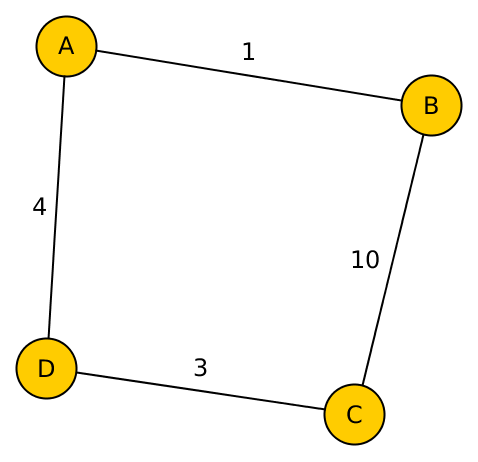
\includegraphics[width=0.6\textwidth]{bilder/distance_vector_example.png}
			\caption{Beispielgraph für Distance Vector}
		\end{minipage}
	\quad
		\begin{minipage}[b]{0.45\linewidth}
			\begin{center}
			\begin{tabular}{ |c|c|c| }
		 	\hline
		 	Ziel & Gewicht & weiter via  \\ 
		 	\hline
		 	A    & -       & -  \\ 
		 	B    & 1       & B  \\ 
		 	C    & 7       & D  \\ 
		 	D    & 4       & D  \\ 
		 	\hline
			\end{tabular}
			\end{center}
		\caption{Distance Vector auf Knoten A}
		\end{minipage}
\end{figure}



Die Einträge für die direkten Nachbarn können sofort erstellt werden. Die Gewichte für die anderen Knoten werden mit ''Infinity'' initialisiert.
Nun werden die Distance Vector Vector Informationen wird rundenbasiert aufgebaut.

In jeder Runde sendet jeder Knoten seine Distance Vector Information an alle direkten Nachbarn.
Sobald ein Knoten eine Distance Vector Nachricht erhalten hat, wird diese ausgewertet. Wenn eine kürzere Route gefunden wurde, wird der entsprechende interne Distance Vector Enitrag aktualisiert.

Um die Distance Vector Tabelle aufzubauen, muss jeder Knoten x $O(d_xn)$ Messages pro Runde verarbeiten ($d_x$ ist Anzahl Kanten des Knoten x). Im gesamten Netzwerk ergibt das $O(nm)$ Messages pro Runde. Der Algorithmus braucht so viele Runden, wie der Durchmesser D des Graphen ist. Somit ergibt sich eine Message Komplexität von $O(Dnm)$ \cite{goodrich2006algorithm}.

Das Routing Infomation Protocol (RIP) \cite{hedrick1988routing} verwendet den Distance Vector Algorithmus.


\section{Unicast Routing mit Link-State}
Ein anderer Algorithmus für Unicast Routing ist Link-State. Die Idee ist, dass in einer ersten Phase alle Knoten die Gewichte ihrer angrenzenden Kanten via Broadcast mit Sequenznummern im Neztwerk bekanntgeben. Danach ist auf jedem Knoten der 'Link-State' aller Knoten gespeichert und mittels dem Algorithmus von Dijkstra werden lokal die kürzesten Wege zu jedem Knoten berechnet und der jeweils erste Knoten im Pfad dahin wird gespeichert.

Das Routing Protocol OSPF \cite{moy1998rfc} ist ein bekanntes Beispiel für Link-State Routing.

Die lokale Berechung mittels einer Standard Implementation von Dijkstra läuft mit Zeitkomplexität $O(m\log{}n)$ \cite{wiki:dijkstra}. Der Speicherverbrauch auf den Knoten ist jeweils $O(n)$.

\newpage

\section{Vergleich von Broadcast und Unicast Algorithmen}

Folgende Tabelle vergleicht die vier beschriebenen Routing Algorithmen bezüglich folgender Kennwerte:
\begin{itemize}
	\item Messages: 		Anzahl Messages, die versendet werden
    \item Lokaler Speicher: Speicher, der auf jedem Knoten benötigt wird
    \item Lokale Zeit: 		Laufzeitverhalten auf den Knoten für die Weiterleitung einer Meldung
    \item Routing Zeit: 	Laufzeitverhalten für die Wegfindung einer Message
\end{itemize}
Der lokale Berechnungsaufwand, der auf den Knoten für den Aufbau von Datenstrukturen benötigt wird, wird hier nicht berücksichtigt. 

\begin{table}[H]
	\centering
		\begin{tabular}{p{0.2\textwidth} p{0.15\textwidth} p{0.15\textwidth} 		   p{0.15\textwidth}       p{0.2\textwidth}} \toprule
            \textbf{Algorithmus} & \textbf{Messages} 	& \textbf{Lokler Speicher} & \textbf{Lokle Zeit}  & \textbf{Routing Zeit} \\ \midrule
			Flooding Hop Counter & $O(1)$      			& $O(1)$ 				   & $O(d)$ 			  & $O((d_{max}-1)^{D})$  \\ \midrule
			Flooding Sequenz Nr. & $O(1)$      			& $O(n)$ 				   & $O(d)$ 			  & $O(m)$  			  \\ \midrule
			Distance Vector		 & $O(Dnm)$    			& $O(n)$ 				   & $O(1)$ 			  & $O(p)$  \\ \midrule
			Link-State			 & $O(m^{2})$  			& $O(n)$ 				   & $O(1)$ 			  & $O(p)$  \\ \midrule
		\end{tabular}
	\caption{Vergleich der asymptotischen Komplexität von statischen Routing Algorithmen \cite{goodrich2006algorithm}}
	\label{tab:diff_routing}
\end{table}

\begin{itemize}
	\item n: Anzahl Knoten im Netz
	\item m: Anzahl Kanten im Netz
    \item d: Maximaler Grad (max. Anzahl Kanten eines Knoten)
    \item D: Durchmesser des Netzwerks
    \item p: Anzahl Knoten des kürzesten Pfades
\end{itemize}

\chapter{Fazit}
\label{chap:schlussfolgerungen}

Verteilte Algorithmen sind in der heutigen Zeit nicht mehr wegzudenken und viele Anwendungen haben sich über viele Jahre und  Jahrzehnte in der Praxis bewährt.

Um die Problemstellungen in verteilten System zu lösen, müssen die Algorithmen spezielle Bedingungen erfüllen. Korrekte und dabei immer noch effiziente Lösungen zu finden, wird besonders bei asynchronen Abläufen schwieriger. 

Es hat sich gezeigt, dass viele Konzepte von sequenziellen Algorithmen übernommen werden können, um ähnliche Probleme in Netzwerken zu lösen. Es sind jedoch zusätzliche Kennwerte für die Komplexitätsanalyse notwendig, um die Algorithmen beurteilen zu können. 

Mit den momentan sehr wichtigen Themen Cloud- und Mobile Computing sind verteilte Systeme und Algorithmen vermehrt wieder relevant geworden in modernen Anwendungen.
%---------------------------------------------------------------------------

% Bibliography
%---------------------------------------------------------------------------
\cleardoublepage
\phantomsection 
\addcontentsline{toc}{chapter}{Literaturverzeichnis}
\bibliographystyle{IEEEtranS}
\bibliography{datenbanken/bibliography}{}
%---------------------------------------------------------------------------

% Listings
%---------------------------------------------------------------------------
\phantomsection 
\addcontentsline{toc}{chapter}{Abbildungsverzeichnis}
\listoffigures
%---------------------------------------------------------------------------


% Attachment:
%---------------------------------------------------------------------------
\appendix
\settocdepth{section}
\chapter{Implementation Leader Election Ring}
\label{chap:app_leaderElection}

Der Sorucecode ist ebenfalls auf folgendem Github Repository verfügbar:\\
\url{https://github.com/barta3/ch.bfh.bti7311.DistributedAlgo}


\lstinputlisting[language=java]{anhang/LeaderElectionRing.java}
\newpage
\lstinputlisting[language=java]{anhang/Message.java}
\newpage
\lstinputlisting[language=java]{anhang/Node.java}

%---------------------------------------------------------------------------

%---------------------------------------------------------------------------
\end{document}